\chapter{Results}\label{chapter:results}

%\section{The issue with inconsistent energy readings} \label{sec:results_the_issue_with_inconsistent_energy_readings}

At the beginning of the experiment, some tools were tested to observe their behavior, understand how to use them, and determine which one best suited the needs of the project.

During the initial testing, a Python framework designed to facilitate experiment measurements was used~\cite{S2_Group_Experiment_Runner}. The framework included an initial test template that used PowerJoular to measure energy of programs. While using the template and testing the framework some bugs and unexpected results were found, some of which were due to misuse of the framework.
Due to these issues, a simpler orchestrator was developed. Although it performed the same core function as the original framework, measuring energy consumption, it was more straightforward, focusing exclusively on energy measurement rather than providing a general-purpose solution. This new orchestrator was implemented in Java.

However, some discrepancies were observed between the energy values measured by the Java and Python frameworks. This was unexpected, as both used the same energy measurement tool (PowerJoular) and measured the same program in the same way. Still, the Python framework consistently reported lower energy values than the Java version.
To investigate which tool was causing the inconsistency, two more orchestrators were implemented. A simplified custom version of the Python framework was also created. In total, four orchestrators were developed: Java, Python, C, and Bash. All four performed the same process, calling PowerJoular to measure the energy usage of a Java program.
This setup represents an early iteration of the approach later detailed in Section~\ref{sec:work_stage2_orchestrator}, which utilized signal-based control to ensure that the measurement tool only ran during the exact computation period being measured.

\begin{figure}[htbp]
  \centering
  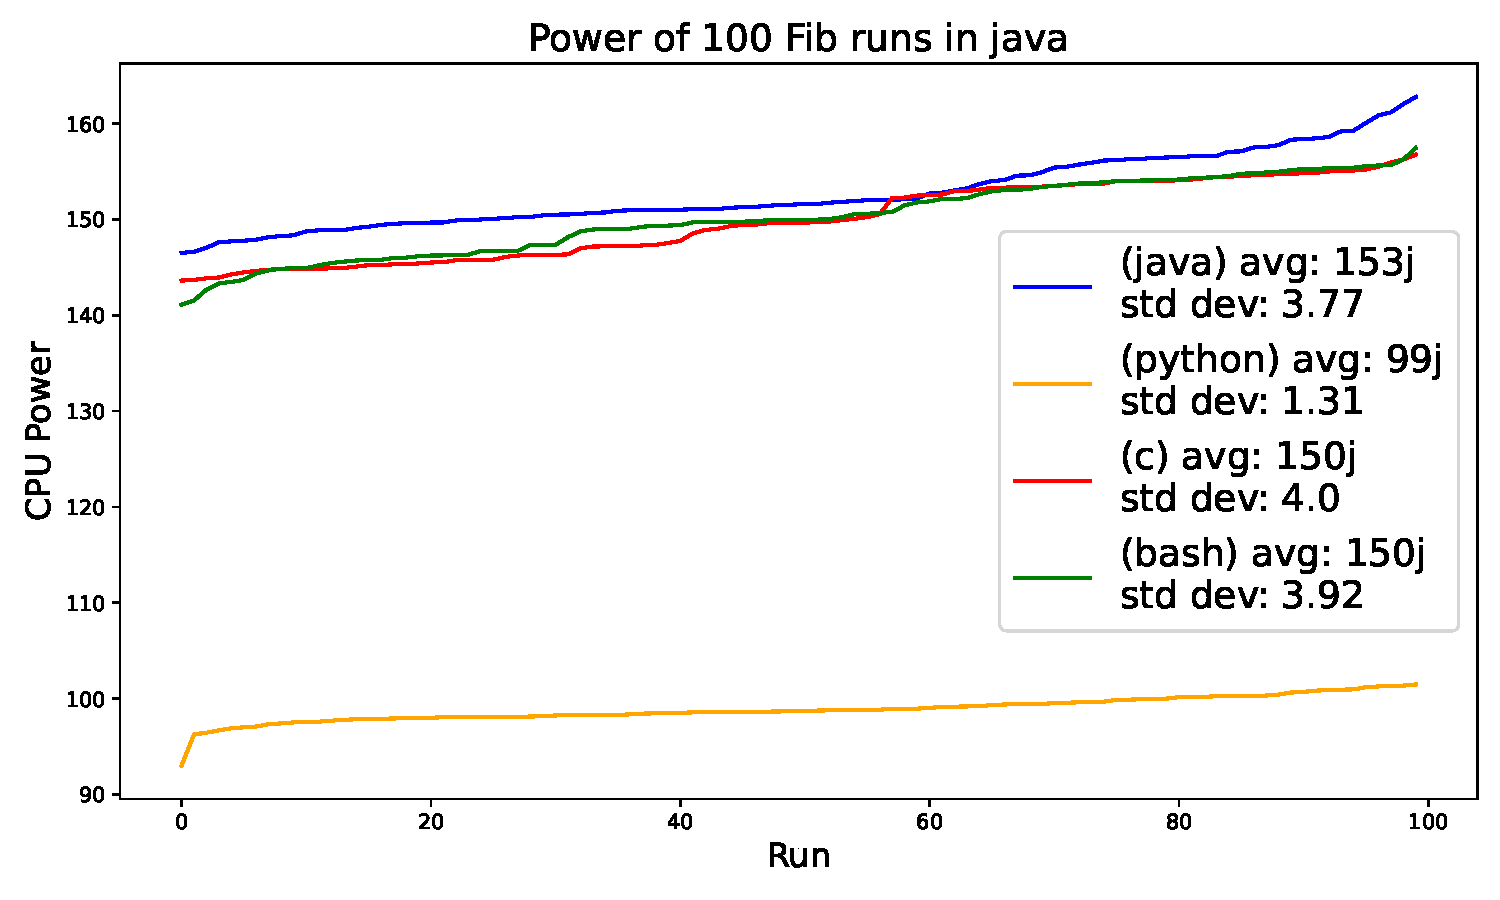
\includegraphics[width = .8 \textwidth]{figures/4_orchs_comparison.pdf}
  \caption{Orchestrators Comparison}
  \label{fig:4_orchs_comparison}
\end{figure}

To better understand the inconsistencies, Figure~\ref{fig:4_orchs_comparison} details the differences.
The figure contains 100 runs of the Fibonacci recursive program written in Java and order by the less energy to the highest energy. And it shows the energy reads for the four different orchestrators used. The labels contain the average energy values and its standard deviation.

It is noticeable that the Python orchestrator read energy values lower than the other orchestrators. Further analysis of the orchestrators revealed a notable difference in behavior. When the Python orchestrator was running, both the parent and child processes consumed CPU resources. In contrast, the other orchestrators (Java, C, and Bash) showed CPU usage only in the child process. This disparity may explain why PowerJoular reported lower energy consumption for the Python orchestrator. Since the CPU load was shared between the parent and child processes, PowerJoular, which measures energy only for the child process (the target Fibonacci program), captured less total energy usage.
Since the experiment runner included an example demonstrating how to use the framework with PowerJoular, the authors were made aware of this potential conflict when launching PowerJoular from Python.


\section{Models Metrics} \label{sec:models_metrics}

For the final version of the tool, models were trained on methods from the Java collections framework, specifically focusing on the \texttt{List} and \texttt{Map} interfaces. Data for these methods was generated, collected, and used to train the models. With the models in place, it is now possible to evaluate their performance using metrics such as R² and Mean Squared Error (MSE), based on the features extracted during data collection.

\begin{figure}[htbp]
  \centering
  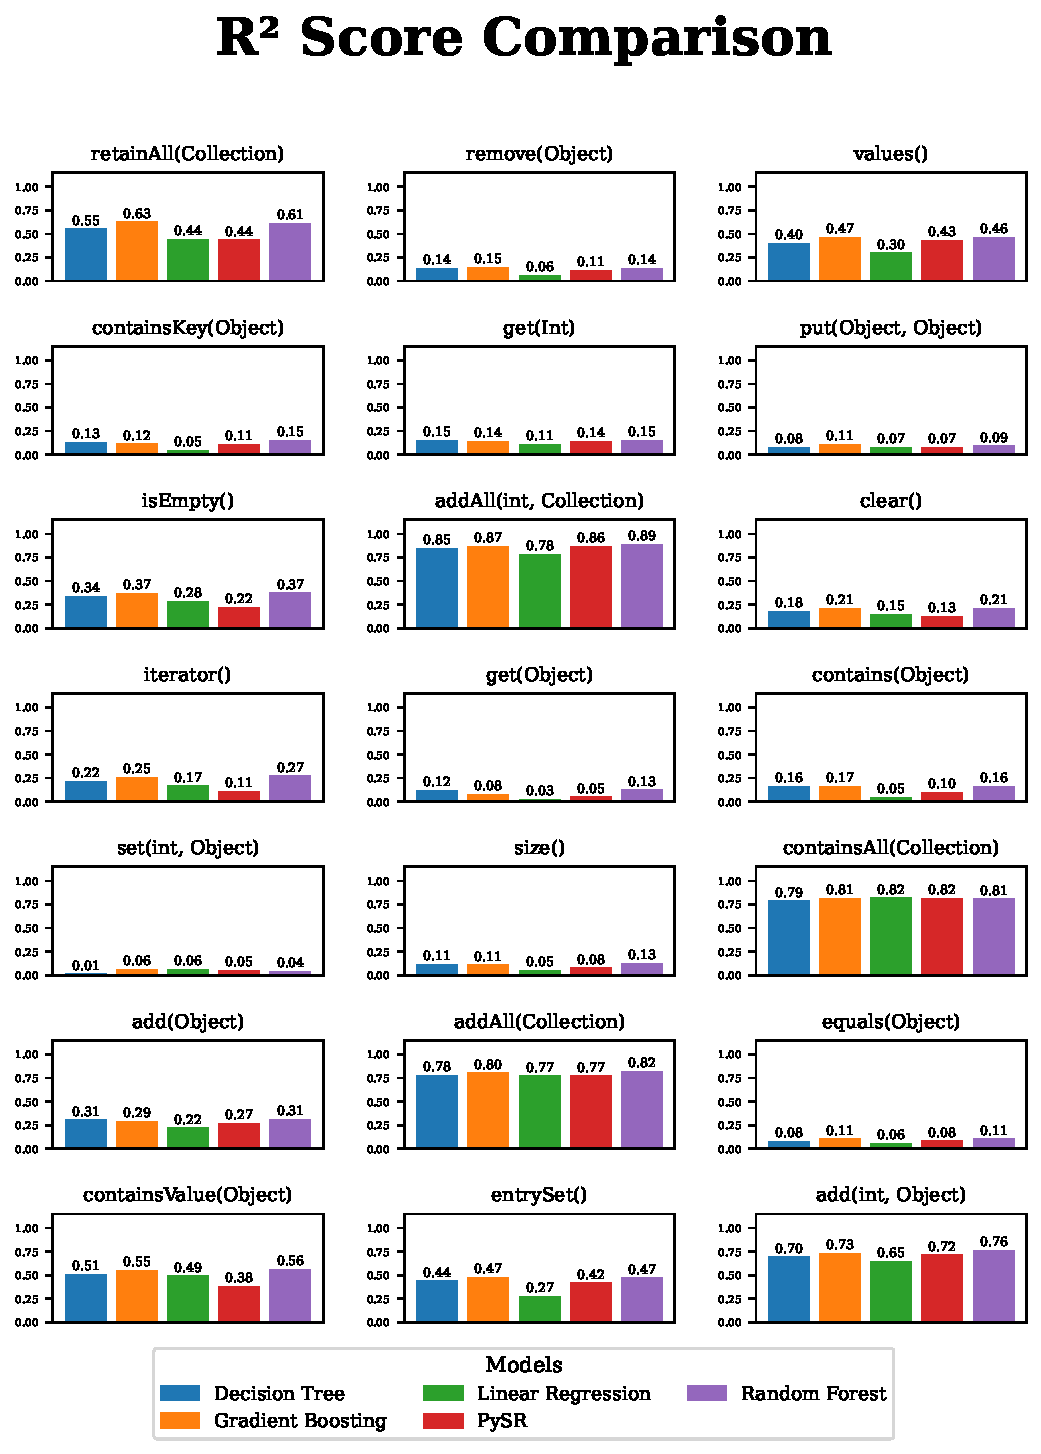
\includegraphics[width=0.85\textwidth]{figures/r2_comparison.pdf}
  \caption{R² Comparison (\textit{Higher is better})}
  \label{fig:r2_comparison}
\end{figure}




\begin{figure}[htbp]
  \centering
  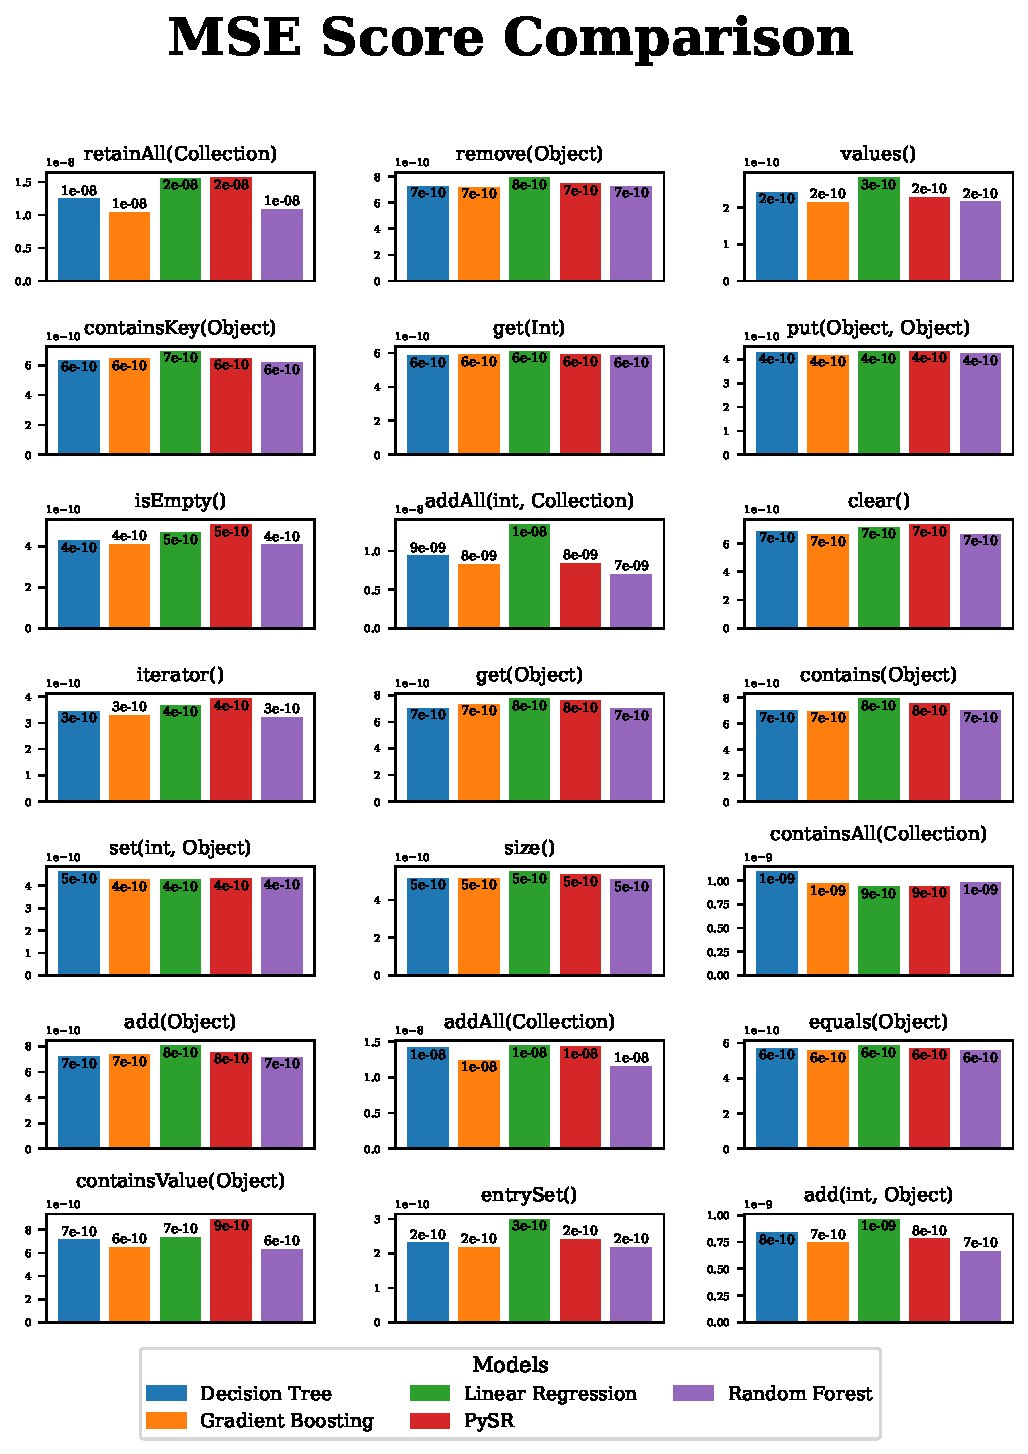
\includegraphics{figures/mse_comparison.pdf}
  \caption{MSE Comparison (\textit{Lower is better})}
  \label{fig:mse_comparison}
\end{figure}

The results of the R² can be seen in the Figure~\ref{fig:r2_comparison}.
Ideally the best score is 1, meaning that the model can get 100\% of the prediction right, however that is not possible in most cases, and this project is not an exception to the rule. It is noticeable that most values are really low (bellow 0.8), which means that the model cannot predict the energy very well for some methods. The best models were for the method \texttt{addAll()} and \texttt{containsAll()} of the List collection, which got an R² of around .8 for most models, meaning that for those 3 methods on average the predictions will be 80\% correct.

For the other methods the scores were lower. The explanation found for this result was the following:


\begin{figure}[htbp]
  \centering
  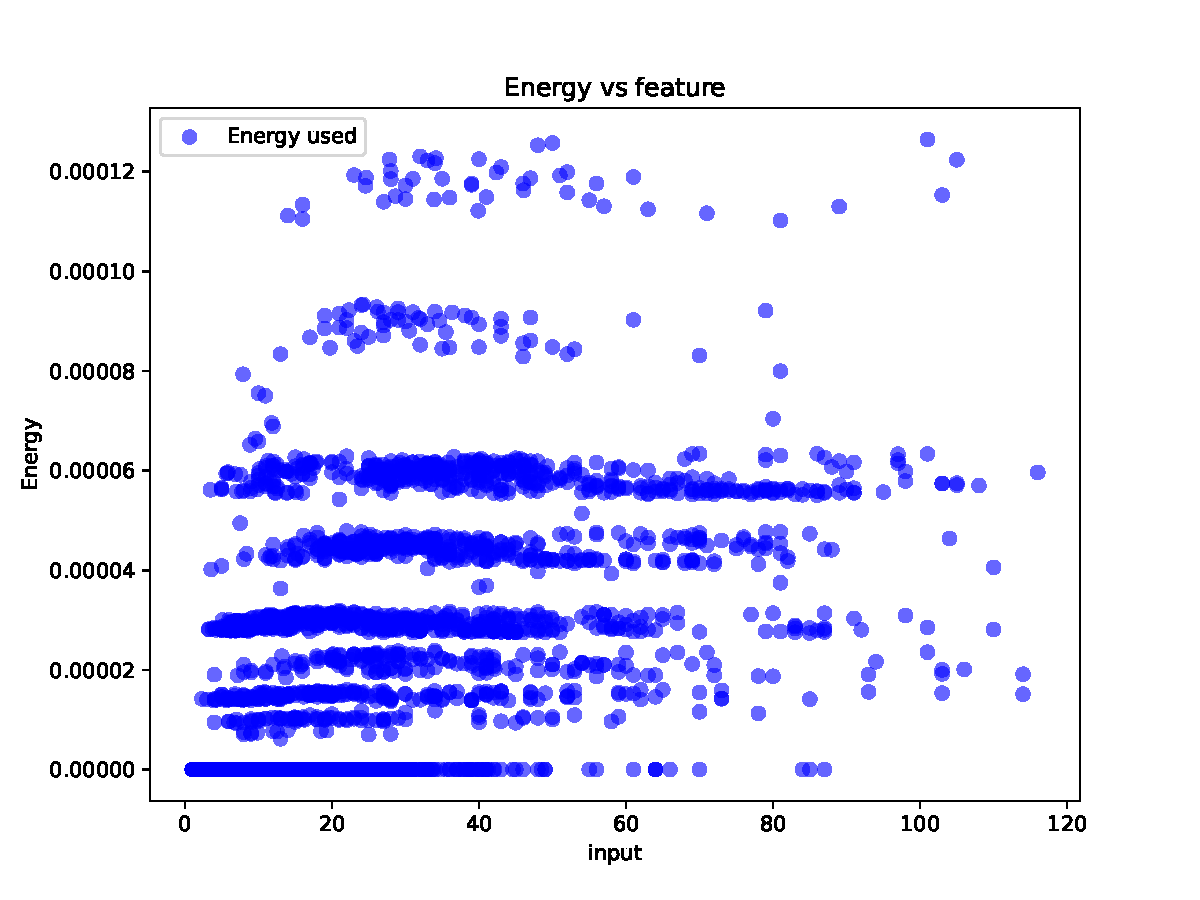
\includegraphics[width = .8 \textwidth]{figures/size_energy.pdf}
  \caption{Energy for the \texttt{List.size()} method with different list sizes.}
  \label{fig:size_energy}
\end{figure}

The 3 methods with the most accuracy were the ones that generated bigger energy outputs, because the methods were computationally more powerful than the others. This made it so that bigger inputs would result in bigger energy outputs, and make the models more easily find a pattern to predict the energy. As for the other models, since a bigger input would not mean a bigger energy output, the model, might had some difficulties predicting the energy. This does not mean that a lower R² will completely make the model unusable for some methods, as their MSE, that can be seen in the Figure~\ref{fig:mse_comparison} is not high, meaning that even when failing to predict the energy of the method, the failed prediction will not be far away as one might expect. For example, if a model has an MSE of $1 \times 10^{-10}$ and predicts the energy usage to be $1~\mathrm{J}$, then even if the prediction is not exact, the true value is likely within $\pm \sqrt{1 \times 10^{-10}} = \pm 1 \times 10^{-5}~\mathrm{J}$ of the prediction, indicating accurate performance despite a potentially low R². 

Another factor that may contribute to low R² scores is the behavior of the energy measurement tool when applied to certain methods. For instance, some methods, such as \texttt{size()}, do not require more computational effort as the collection size increases. Whether the collection has one element or one million, the method executes in roughly the same amount of time. Consequently, the energy consumption remains nearly constant, regardless of the input size. Since these methods complete very quickly and consume very little energy, even minimal measurement noise can significantly affect the recorded values. Figure~\ref{fig:size_energy} illustrates this effect: although an increase in energy with input size is typically expected, the recorded energy values for \texttt{List.size()} remain considerably flat. While this example isolates a single feature, and other features also influence energy consumption, input size is often the most significant. This observation suggests that for low-energy, low-variance methods, measurement noise can impact the signal, making accurate energy prediction particularly challenging.


Nonetheless, the lower R² scores should be addressed, and what can be done to improve the results of these models is to have the program generator create higher inputs, so the energy profiles also have outputs with higher energy, making the energy predictions more accurate. Then, since most of the predictions depend on the input, it means the other features do not have such higher impact, so it is also important to pick better features and remove others that might not be interesting. 



In general, most of the models present similar scores, however the chosen one was PySR. As it can represent the predictions in expressions which can help the users to try to understand why the code is using more energy. It has a nice feature of allowing to balance complexity and accuracy. And can easily be used in another code language as it is represented as a mathematical expression.
The fact that most models present similar results, ranging from advanced models like Random Forest and Gradient Boosting to simple models like Linear Regression, suggests that features used in the model likely do not capture highly nonlinear or complex relations. This indicates that energy consumption behavior in analyzed approaches can be reliably captured by simple relations. As a result, the set of features cannot offer the richness or variability needed for distinguishing more subtle energy behavior. This does not mean that the learning problem is simple, rather, it indicates that the available features may fail to express potential nonlinear patterns of energy consumption. To improve prediction performance and enable more effective use of expressive models, future work should incorporate features capable of highlight the complexity of predicting energy usage.



\section{Predicted vs. Measured Energy} \label{sec:predicted_vs_measured_energy}

Since the extension has been built, we can present the results and evaluate how accurately the tool estimates energy consumption compared to real measurements obtained using PowerJoular. Since the energy profiles were generated on a specific hardware setup (see Table~\ref{tab:hardware_specs}), the resulting models are adjusted to that particular system. If the tool were run on a different machine, the absolute energy values would likely differ due to variations in hardware characteristics. However, the relative differences in energy consumption between operations are expected to remain consistent. For instance, if \texttt{TreeMap} consumes more energy than \texttt{HashMap} on one system, the same trend will likely hold on another system, even if the exact energy values vary.

\begin{listing}[H]
\noindent\rule{\linewidth}{0.4pt}
\begin{minted}[linenos, fontsize=\small, frame=none, bgcolor=white,breaklines=true,breakanywhere=true]{Java}
    ArrayList<Integer> l = new ArrayList<>();
    ArrayList<Integer> l2 = new ArrayList<>();
    l.addAll(l2);
\end{minted}
\noindent\rule{\linewidth}{0.4pt}
\caption{Code example}            
\label{lst:code_example}
\end{listing}

To test if the extension tool is accurate, the energy measurement needs to be run in the same machine were the data was collected.
For this a simple program was developed, Listing~\ref{lst:code_example}, more like simple Java instructions, of just creating two lists (both with size 1000) and using the method \texttt{addAll(Object)} and checking if the prediction matches the actual measurement.

\begin{table}[htbp]
  \centering
  \label{tab:energy_comparison}
  \footnotesize
  \begin{tabular}{>{\raggedright\arraybackslash}p{4cm}ccc}
    \toprule
    Method & Actual Energy Range (J) & Predicted Energy (J) & Prediction Error (\%) \\
    \midrule
    \texttt{addAll(Object)} & 4.9e-4 -- 5.1e-4 & 5.51e-4 & 10.2 \\
    \midrule
    \texttt{addAll(Object)} + \texttt{size()} + \texttt{equals(Object)} & 5.0e-4 -- 5.2e-4 & 6.49e-4 & 27 \\
    \midrule
    \texttt{Map.put(Object, Object)} + \texttt{loop(1000)} & 0.0027 -- 0.0030 & 0.033 &  1058 \\
    \bottomrule
  \end{tabular}
  \vspace{0.5em}
  \caption{Comparison of actual and predicted energy consumption for different methods}
  %\footnotesize{The actual energy ranges were obtained by running the program 10 times.}
\end{table}


%\begin{table}[htbp]
%  \centering
%  \footnotesize
%  \makebox[\textwidth][c]{%
%    \begin{tabular}{@{}p{5cm}@{\hspace{2.5em}}c@{\hspace{0.5em}}ccc@{}}
%      \toprule
%      Method & Actual Energy Range (J) & Predicted Energy (J) & Input Value (\%) & Prediction Error (\%) \\
%      \toprule
%      \texttt{BinaryTrees.createTree(int)} & 3.75e-4 -- 4.60e-4 & -0.083 & 10 & 19980 \\
%      \midrule
%      \texttt{BinaryTrees.createTree(int)} & 11.78 -- 12.63 & 10.26 & 23 & 15.9 \\
%      \midrule
%      \texttt{BinaryTrees.createTree(int)} & 77.29 -- 80.63 & 79.90 & 26 & 1.2 \\
%      \midrule
%      \texttt{BinaryTrees.checkTree(TreeNode)} & 1.64e-4 -- 1.75e-4 & 1.88e-4 & 10 & 10.9 \\
%      \midrule
%      \texttt{BinaryTrees.checkTree(TreeNode)} & 1.37 -- 1.56 & 2.19e-3 & 23 & 99.85 \\
%      \midrule
%      \texttt{BinaryTrees.checkTree(TreeNode)} & 11.72 -- 13.29 & 3.15e-3 & 26 & 99.97 \\
%      \midrule
%      \texttt{BinaryTrees.trees(int)} & 0.041 -- 0.045 & -3.42 & 10 & 127 \\
%      \midrule
%      \texttt{BinaryTrees.trees(int)} & 713 -- 800 & 517.89 & 23 & 31.59 \\
%      \midrule
%      \texttt{BinaryTrees.trees(int)} & 6260 -- 7111 & 2429 & 26 & 63.66 \\
%      \midrule
%      \texttt{BinaryTrees.checkTree(TreeNode) + createTree(int) + trees(int)} & 4.59e-2 -- 4.77e-2 & -3.49 & 10 & 7578 \\
%      \midrule
%      \texttt{BinaryTrees.checkTree(TreeNode) + createTree(int) + trees(int)} & 796 -- 806 & 528.15 & 23 & 34.08 \\
%      \midrule
%      \texttt{BinaryTrees.checkTree(TreeNode) + createTree(int) + trees(int)} & 7062 -- 7350 & 2509 & 26 & 65.18 \\
%      \bottomrule
%    \end{tabular}%
%  }
%  \caption{Comparison of actual and predicted energy consumption for BinaryTrees program}
%  \label{tab:energy_comparison_bin_trees}
%\end{table}







The actual value measured by PowerJoular is in the range of 4.9e-4 to 5.1e-4J while the prediction is 5.51e-4J. This shows that the prediction was good for this method in particular.
When trying to add two more operations (\texttt{size()} and \texttt{equals(Object)}) the measurement is in the range of 5.0e-4 to 5.2e-4J and the prediction is 6.49e-4J, so now the values are getting off. The method \texttt{addAll(Object)} is one of the methods that has the best accuracy of around 80\%, and the other two do not. This makes it so that when adding the other two methods the real energy value starts drifting away from the real one.

This can get worse when the number of methods used and variables involved start increasing, leading to greater divergence between the prediction output and actual values. 

Using the example of the word counting program, Listing~\ref{lst:Java_program_to_count_word_frequencies_in_a_string}, which involves Maps and loops, the bigger gap between reality and prediction can be seen, as the Map methods predictions are not very accurate. The loop has a size of 1000 (extension default) and the Map contains 3 unique entries, since the input string includes just three distinct words.

The energy measured is in the range of 0.0027J to 0.0030J and the prediction is 0.033J. This deviates by a factor of 10 which is considerable and makes the prediction absolute values not viable. However, the relative predictions remain consistent, as input sizes increase, the predicted energy consumption also increases.

Another problem is that summing the predictions of individual methods can lead to error accumulation, which increases discrepancies between predicted and actual energy values as more methods are used, even if the individual models are accurate. To mitigate this, one potential solution is to introduce a correction factor or calibration step based on empirical error measurements, adjusting the final predicted value to better reflect observed trends.

The results demonstrate that while the tool provides useful estimations of energy consumption, especially in terms of relative trends between methods and input sizes, its absolute predictions can vary significantly depending on the type of operations being analyzed. Additionally, while some methods show high prediction accuracy (e.g., addAll(Object)), combining multiple methods or increasing program complexity tends to amplify prediction errors. These limitations highlight the importance of carefully selecting input sizes and operations for meaningful energy analysis, and they suggest that the tool is best suited for relative comparisons rather than precise energy estimation.


\begin{figure}[htbp]
  \centering
  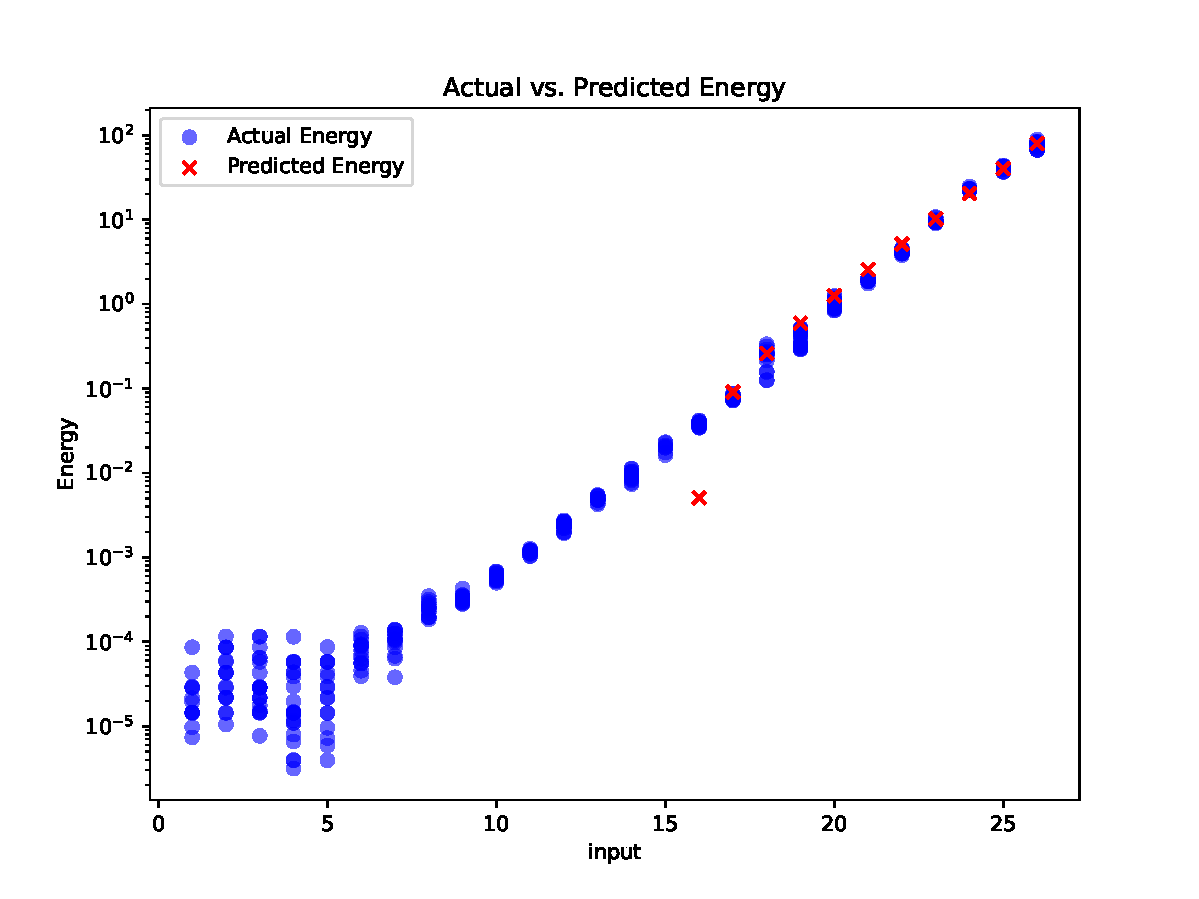
\includegraphics[width = .7 \textwidth]{figures/createTree_plot.pdf}
  \caption{Energy for method \texttt{createTree}}
  \label{fig:createTree_plot}
\end{figure}

\begin{figure}[htbp]
  \centering
  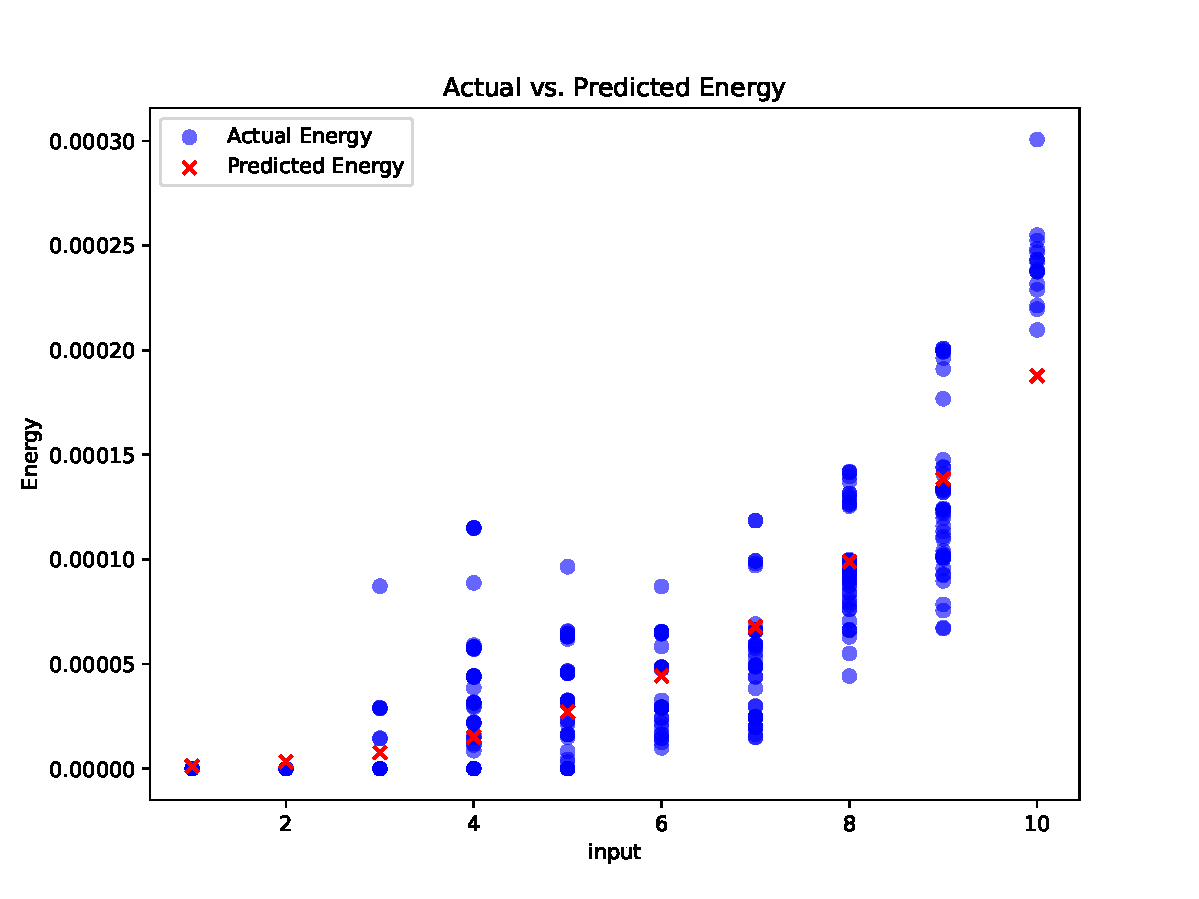
\includegraphics[width = .7 \textwidth]{figures/checkTree_plot.pdf}
  \caption{Energy for method \texttt{checkTree}}
  \label{fig:checkTree_plot}
\end{figure}

\begin{figure}[htbp]
  \centering
  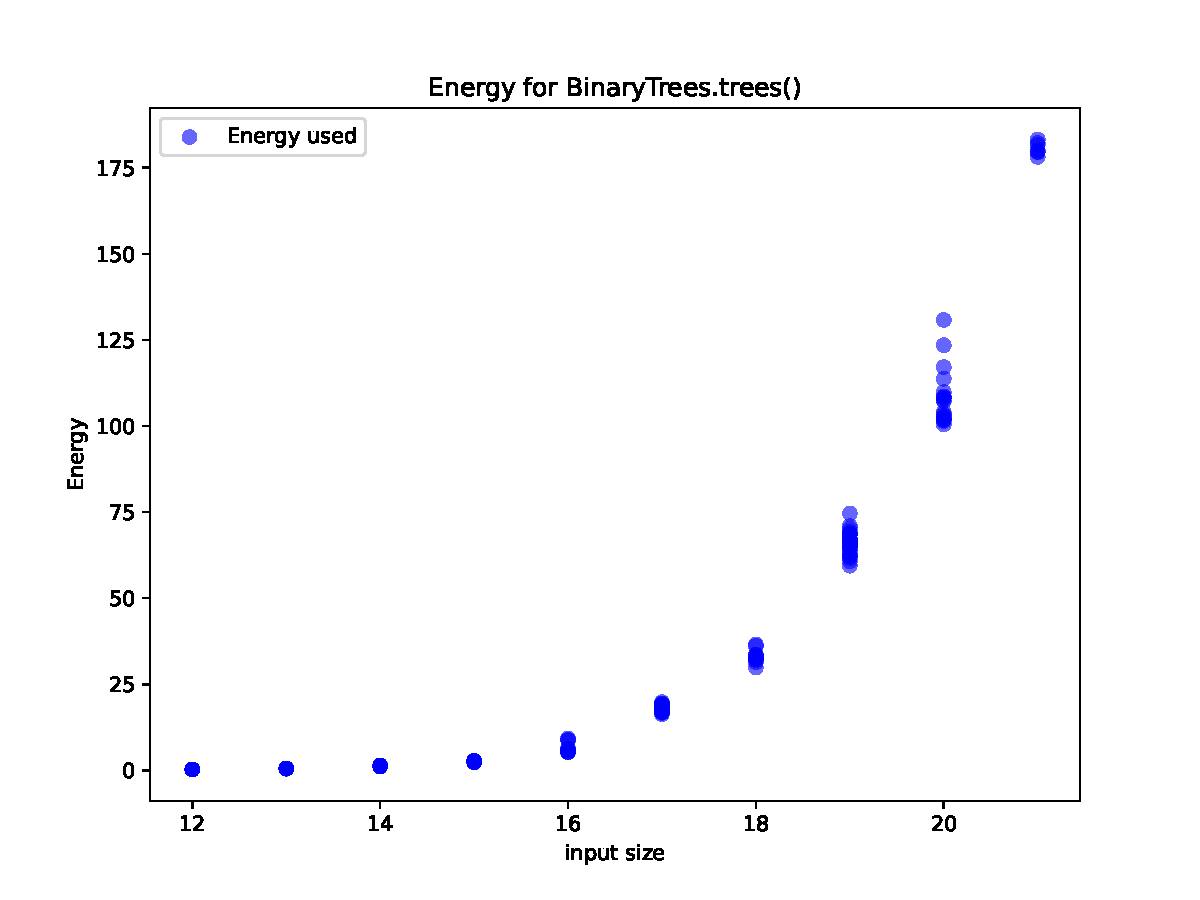
\includegraphics[width = .7 \textwidth]{figures/trees_plot.pdf}
  \caption{Energy for method \texttt{trees}}
  \label{fig:trees_plot}
\end{figure}


{\color{blue}
  Another experiment was conducted using a test case considered more realistic than the others. The program was selected from the Computer Language Benchmarks Game, which provides algorithmic benchmarks designed to test language performance on tasks that are representative of certain real-world computational workloads~\cite{benchmarksGameJava}.

The program selected was the \texttt{}{BinaryTrees} (Java naot #3), which are computational intensive task. It contains three core methods, described as follows:


\begin{itemize}
  \item \textbf{createTree:} Recursively builds a binary tree of the given depth. At each level, creates a node with two children (left and right), until depth equals zero. The result is a complete binary tree with \(2^{\text{depth}} - 1\) nodes.
 
  \item \textbf{checkTree:} Recursively traverses the tree and counts the number of nodes. For leaf nodes, it returns \texttt{1}. For internal nodes, it returns the sum of the recursive calls on the left and right subtrees plus one: $1 + \text{check(left)} + \text{check(right)}$.
  
  \item \textbf{trees:} Performs the core part of the benchmark by creating and checking many binary trees of varying depths and keeping one long-lived tree in memory to simulate memory pressure.
\end{itemize}
}

{\color{blue}
  The Figures~\ref{fig:createTree_plot},~\ref{fig:checkTree_plot}, and~\ref{fig:trees_plot} show the energy of each method, for different input sizes, for every program generated and analyzed by the framework. It is possible to see that the methods have an exponential tendency with the increase of the input, which is expected from binary trees operations. It is also noticeable that the Figure~\ref{fig:checkTree_plot} has a lower curve and input, this was due to the fact that the method required that a tree was created before the method could be run, which would take more time, subsequently, the maximum input for this method was lower. 


From how the program is implemented on the website it needs some small adjustments in order to work with our framework. First, the program does not have a constructor for the class \texttt{TreeNode} which does not allow the program generator to populate the programs correctly, as the program on the website uses a custom method that create the nodes. Without this change, the methods that required \texttt{TreeNode} as input would be simply receiving an empty Object, as the constructor was also empty, making their generation useless as every program would be the same.
With that said, the only adjustments made to the class were, a new private empty constructor, that can only be accessed inside the class, so the generator does not detect it and use it, as the generator always tries to use the smallest one available, so it is important that the empty constructor is private. And it was added a new constructor, this one public, that had the same logic as the method that created the nodes. Now the methods that use \texttt{TreeNode} can be generated as the constructor can call the public constructor that has the similar behavior of the \texttt{createTree(int)} method. These changes do not impact how the program, or methods behave and only helps the program generation.

After that the data was collected and the models for each method used in the program was trained.
}

\begin{table}[htbp]
  \centering
  \footnotesize
  \setlength{\tabcolsep}{10pt} % increase column separation
  \makebox[\textwidth][c]{%
    \begin{tabular}{@{}p{5.3cm}@{\hspace{2.5em}}c@{\hspace{1em}}c@{\hspace{1em}}c@{\hspace{1em}}c@{}}
      \toprule
      Method & Input Value & Predicted Energy (J) & Actual Energy Range (J) & Prediction Error (\%) \\
      \toprule

      \multirow{3}{*}{\texttt{BinaryTrees.createTree(int)}} 
        & 10 & -0.083 & 3.75e-4 -- 4.60e-4 & 19980 \\
        & 23 & 10.26 & 11.78 -- 12.63 & 15.9 \\
        & 26 & 79.90 & 77.29 -- 80.63 & 1.2 \\
      \midrule

      \multirow{3}{*}{\texttt{BinaryTrees.checkTree(TreeNode)}}
        & 10 & 1.88e-4 & 1.64e-4 -- 1.75e-4 & 10.9 \\
        & 23 & 2.19e-3 & 1.37 -- 1.56 & 99.85 \\
        & 26 & 3.15e-3 & 11.72 -- 13.29 & 99.97 \\
      \midrule

      \multirow{3}{*}{\texttt{BinaryTrees.trees(int)}}
        & 10 & -3.42 & 0.041 -- 0.045 & 8053 \\
        & 23 & 517.89 & 713 -- 800 & 31.59 \\
        & 26 & 2429 & 6260 -- 7111 & 63.66 \\
      \midrule

      \multirow{3}{*}{\shortstack[l]{\texttt{BinaryTrees.checkTree(TreeNode)} +\\\texttt{createTree(int)} +\\\texttt{trees(int)}}}
        & 10 & -3.49 & 4.59e-2 -- 4.77e-2 & 7578 \\
        & 23 & 528.15 & 796 -- 806 & 34.08 \\
        & 26 & 2509 & 7062 -- 7350 & 65.18 \\
      \bottomrule
    \end{tabular}%
  }
  \caption{Comparison of actual and predicted energy consumption for BinaryTrees program}
  \label{tab:energy_comparison_bin_trees}
\end{table}



%\begin{table}[htbp]
%  \centering
%  \footnotesize
%  \setlength{\tabcolsep}{10pt}
%  \makebox[\textwidth][c]{%
%    \begin{tabular}{@{}p{5.3cm}@{\hspace{2em}}c@{\hspace{1em}}c@{\hspace{1em}}c@{\hspace{1em}}c@{}}
%      \toprule
%      Method & Input Value (\%) & Predicted Energy Simple Model (J) & Predicted Energy Best Model (J) & Actual Energy Range (J) & Prediction Error Simple Model (\%) & Prediction Error Best Model (\%) \\
%      \toprule
%
%      \multirow{3}{=}{\texttt{BinaryTrees.createTree(int)}} 
%        & 10 & -0.083 & 5.63e-04 & 3.75e-4 -- 4.60e-4 & 19980 & 34.97 \\
%        & 23 & 10.26 & 9.42 & 11.78 -- 12.63 & 15.9 & 22.83 \\
%        & 26 & 79.90 & 80.11 & 77.29 -- 80.63 & 1.2 & 1.45 \\
%      \midrule
%
%      \multirow{3}{=}{\texttt{BinaryTrees.checkTree(TreeNode)}}
%        & 10 & 1.88e-4 & 2.28e-04 & 1.64e-4 -- 1.75e-4 & 10.9 & 34.4 \\
%        & 23 & 2.19e-3 & 2.43e-03 & 1.37 -- 1.56 & 99.85  & 99.83\\
%        & 26 & 3.15e-3 & 3.53e-03 & 11.72 -- 13.29 & 99.97 & 99.97\\
%      \midrule
%
%      \multirow{3}{=}{\texttt{BinaryTrees.trees(int)}}
%        & 10 & -3.42 & 1.69 & 0.041 -- 0.045 & 8053 & 3833 \\
%        & 23 & 517.89 & 798 & 713 -- 800 & 31.59 & 5.49\\
%        & 26 & 2429 & 39754 & 6260 -- 7111 & 63.66 & 494.63 \\
%      \midrule
%
%      \multirow{3}{=}{\parbox{5.3cm}{\centering\texttt{BinaryTrees.checkTree(TreeNode) +\\ createTree(int) + trees(int)}}}
%        & 10 & -3.49 & 4.59e-2 -- 4.77e-2 & 7578 \\
%        & 23 & 528.15 & 796 -- 806 & 34.08 \\
%        & 26 & 2509 & 7062 -- 7350 & 65.18 \\
%      \bottomrule
%    \end{tabular}%
%  }
%  \caption{Comparison of actual and predicted energy consumption for BinaryTrees program}
%  \label{tab:energy_comparison_bin_trees}
%\end{table}



{\color{blue}
The results are detailed in the Table~\ref{tab:energy_comparison_bin_trees}. 

It is noticeable that the values predicted are not the most accurate, for some inputs it has good accuracy, for example, the method \texttt{createTree} has good accuracy for the input \texttt{26}. For other methods, like \texttt{trees} it does not. Again as the previous experiment, the tool is not very accurate in terms of absolute values, and in this case for methods that change their energy considerably with minimum increase in the input, the models have a harder time to predict. The tool demonstrates good relative energy prediction, as input values increase, the predicted energy consumption also increases, and it decreases correspondingly when the inputs are reduced.

To achieve better results with the \texttt{BinaryTrees} methods it could be possible to improve the feature's selection by incorporating characteristics that better capture the program complexity and increase the maximum input available for each program generated in order to better represent the high-energy regions of execution.

However, this experiment objective's was not focused only on achieving the highest accuracy possible. It was also made to prove that it is possible to use the framework to test more interesting and complex cases. And it was proven that with minimal changes, it was possible to mass generate programs, collect data and train models, for the \texttt{BinaryTrees} program. While it may not work universally for all programs, since creating a framework general enough to handle every case is challenging, this experiment demonstrates that analyzing custom programs is possible.
}





\section{Limitations and Challenges} \label{sec:limitations_and_challenges}

During program generation, most of the tested collections focused on List, Set, and Map. However, programs were also generated for another collection category, the Math collection. This introduced an issue. The computations in these programs were extremely fast, completing too quickly for PowerJoular to measure any meaningful energy consumption. As a result, all energy readings for the Math collection programs were reported as 0J.
The problem was the array sizes used to hold the method parameters. While the three predefined array sizes worked well for List, Set, and Map collections, they were too small for the Math collection. The smaller input sizes caused the Math computations to execute very fast, not giving PowerJoular enough time to capture energy usage.
This highlights a challenge in energy profiling: some collections, especially those involving lightweight or highly optimized operations like Math functions, may be difficult to measure accurately. One possible solution would be to determine array sizes during program generation, large enough to ensure that each program runs for at least one second, giving PowerJoular sufficient time to measure energy consumption. However, implementing this would significantly increase the time required for program generation, as it would involve exploring many more combinations of input sizes to find suitable configurations.


Another important factor is that the tool is not able to predict energy when threads are involved, as the programs generated only used a single thread, subsequently the models will not have that factor into account. This limitation exists because measuring and modeling the energy usage of multithreaded programs is particularly challenging due to factors like concurrent execution, thread scheduling, and synchronization overhead. However, threading can deeply impact the energy usage of a program, as a program execution stop being strictly linear, and can have multiple simultaneous computations, potentially increasing the code energy consumption.

{\color{blue}
  A limitation detected during the experimentation of analyzing an external program, was how the inputs on some programs are defined. For example, a program can have a method that receives a String, however, when inside the method it decides to convert the String to int and use it as an Integer, making it so a method that actually uses Integers and not Strings. Although it is easily noticeable by human eye, the program generator cannot understand this kind of context changes as easy, and it would start generating inputs for Strings instead of Integers, which would fail in the program generation. A good example of this usage is when the main function is called and receives the arguments in the \texttt{String[]} and then it uses its values in different variables.
}




%In the start of the project, some tools were tested in order to see how to get the energy profiles for later use. The tools tested were PowerJoular, Powertop, Perf and JoularJx.
%
%Perf is a Linux tool primarily designed for analyzing application performance characteristics rather than precise energy measurement. While it can provide some energy-related metrics, its measurements tend to be imprecise. In this context, Perf was used mainly to get a rough idea of energy consumption and to serve as an alternative when more accurate tools were unavailable.
%
%Powertop was also tested, but it could only perform energy measurements on laptops, as it relies on battery drain data to calculate energy consumption. Since this approach doesn't align with our specific requirements, we considered Powertop as a last-resort option.
%
%JoularJx is an energy measurement tool capable of measuring the consumption of Java programs and its methods. However, it is not as precise as other tools as it requires to measure the entire start of the JVM and whole functions instead of small code blocks.
%
%As described in the \ref{sec:background_energy}, PowerJoular is the best option. As a command line program it can be easily adapted to measure any program or code snippet in most languages. So it was combined with the framework experiment-runner, that facilitates the process.
%
%Initially, JoularJx and the experiment-runner using PowerJoular were used to explore their capabilities and familiarize with the tools. A sample Fibonacci program written in Java and C was used as a test case. However, the energy measurements provided by the two tools differed, and the experiment runner occasionally encountered errors. Later, it was determined that these problems were due to incorrect use of the framework. However, it was still decided the best approach was to make a new orchestrator similar to the Experiment-Runner, but simpler and specifically focused on measuring process energy consumption using PowerJoular. A Java-based orchestrator was initially developed because the Fibonacci implementation was also in Java. However, when tested, the energy measurement results differed significantly from those of the experiment runner, even though the main difference was the programming language (Java vs. Python).
%
%To further analyze these inconsistencies, another orchestrator was developed in Python. This allowed for a closer examination of the differences in energy measurements and a deeper understanding of the behavior of the tools.
%
%Using the process explained on \ref{chapter:approach} it was noticeable that the Java orchestrator was getting significantly more energy consumption than the Python one, which is not very logical, since they both target the same program. So, to try and check which one was having problems, two more orchestrators were implemented, one in C and another in bash.
%
%After running the tests again it was possible to see that the Python orchestrator was getting values way more different from the other three orchestrators as show in Figure \ref{fig:4_orchs_comparison}.
%The figure contains 100 runs of the Fibonacci recursive program written in Java and order by the less energy to the highest energy. And it shows the energy reads for the four different orchestrators used. The labels contain the average energy values and its standard deviation.
%
%Further analysis of the orchestrators revealed a notable difference in behavior. When the Python orchestrator was running, both the parent and child processes consumed CPU resources. In contrast, the other orchestrators (Java, C, and Bash) showed CPU usage only in the child process. This disparity may explain why PowerJoular reported lower energy consumption for the Python orchestrator. Since the CPU load was shared between the parent and child processes, PowerJoular, which measures energy only for the child process (the target Fibonacci program), captured less total energy usage.
%Since the experiment runner included an example demonstrating how to use the framework with PowerJoular, the authors were made aware of this potential conflict when launching PowerJoular from Python.
%
%\begin{figure}%[h]
%  \centering
%  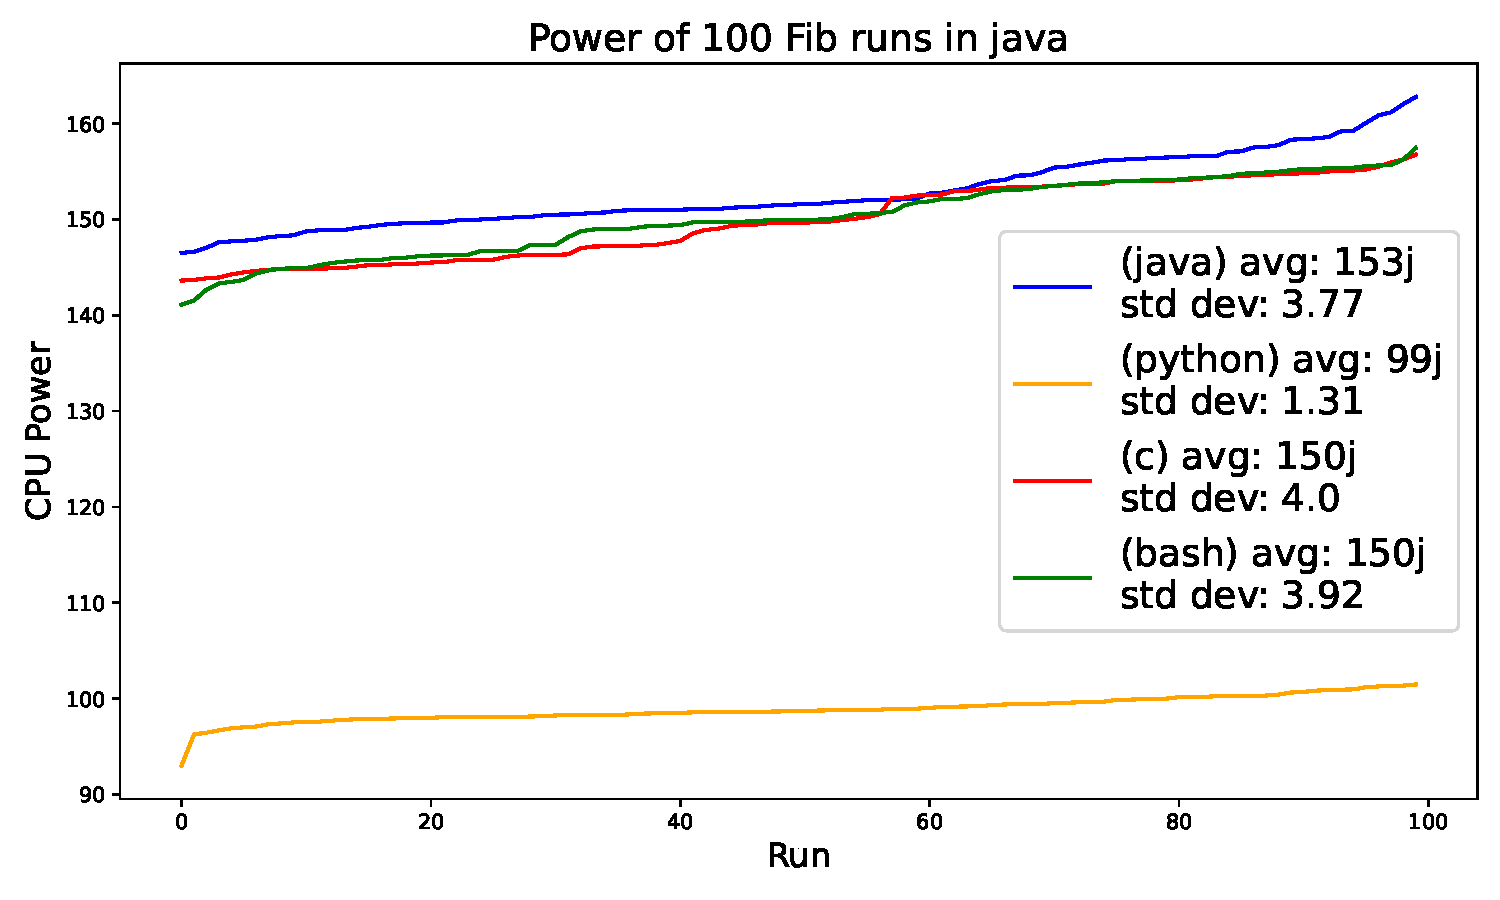
\includegraphics[width = 0.5 \textwidth]{figures/4_orchestrators_comparison.pdf}
%  \caption{orchestrators comparison}
%  \label{fig:4_orchs_comparison}
%\end{figure}